\documentclass[10pt]{beamer}

% Fira Sans/Mono/Math are installed in ~/.local/share/fonts (copied from
% texmf, registered with fontconfig), so the focus theme can use its
% intended Fira fonts -- real sans + small caps, no serif fallback.
\usetheme{focus}

% --- colour palette -------------------------------------------------------
\definecolor{inkblack}{HTML}{0D1B2A}      % deepest: frametitle / section band
\definecolor{main}{HTML}{1B263B}          % Prussian Blue: body text, blocks
\definecolor{background}{HTML}{E0E1DD}     % Alabaster Grey: slide background
\definecolor{alert}{HTML}{415A77}          % Dusk Blue: accent / links / cites
\definecolor{example}{HTML}{778DA9}        % Dusty Denim: example blocks
\setbeamercolor{titlelike}{fg=background, bg=inkblack}
% -------------------------------------------------------------------------

\usepackage{appendixnumberbeamer}

\usepackage{booktabs}
\usepackage{array,multirow}
\usepackage[authoryear,round]{natbib}

\usepackage{amsmath,mathtools}   % amssymb dropped: focus loads unicode-math

\usepackage{pgfplots}
\usepgfplotslibrary{dateplot}

\usepackage{tikz}
\usetikzlibrary{arrows.meta,positioning}
\usepackage{float, graphicx}
\graphicspath{{figures/}}

% Accent for links and citations: the focus theme's alert color.
\hypersetup{
  colorlinks=true,
  linkcolor=alert,
  citecolor=alert,
  urlcolor=alert
}
% natbib + hyperref only color the linked tokens, leaving the round
% parentheses uncolored. Wrap \citet so the whole citation (incl.
% parentheses) takes the accent color.
\AtBeginDocument{%
  \let\focusoldcitet\citet
  \renewcommand{\citet}[1]{\textcolor{alert}{\focusoldcitet{#1}}}%
}

% --- notation shortcuts ---------------------------------------------------
\newcommand{\E}{\mathbb{E}}
\newcommand{\pt}{\widetilde{\pi}}
\newcommand{\rSS}{\mathrm{SS}}
\newcommand{\rUI}{\mathrm{UI}}
\newcommand{\rIU}{\mathrm{IU}}
\newcommand{\Vhat}{\widehat{V}_U}
\newcommand{\timinggametable}[4]{%
  \begin{table}[H]
    \setlength{\extrarowheight}{3pt}
    \centering
    \begin{tabular}{cc|c|c|}
      & \multicolumn{1}{c}{} & \multicolumn{2}{c}{Agent $U$}\\
      & \multicolumn{1}{c}{} & \multicolumn{1}{c}{Period 1} & \multicolumn{1}{c}{Period 2} \\\cline{3-4}
      \multirow{2}*{Agent $I$} & Period 1 & #1 & #2 \\\cline{3-4}
      & Period 2 & #3 & #4 \\\cline{3-4}
    \end{tabular}
  \end{table}%
}
\setbeamertemplate{theorems}[numbered]

% Breakable proof: beamer's proof is a non-breakable block, so a long
% proof overflows instead of flowing across allowframebreaks pages.
% This plain version flows freely; the QED square appears only once,
% at the very end of the proof.
\renewenvironment{proof}{%
  \par\smallskip\noindent\textit{Proof.}\hspace{0.6em}\ignorespaces
}{%
  \unskip\nobreak\hfill$\square$\par\smallskip
}
% -------------------------------------------------------------------------

% The focus title template gives title/subtitle fixed-height boxes;
% scale these fonts down so the long title and subtitle do not overflow
% into the author line.
\setbeamerfont{title}{size=\LARGE, series=\bfseries, shape=\scshape}
\setbeamerfont{subtitle}{size=\normalsize, shape=\scshape}
\setbeamerfont{institute}{size=\small, shape=\scshape}

\title{Separation, Pooling,\\ and Endogenous Timing}
\subtitle{A Tullock Contest under Two-sided Asymmetry}
\date{\today}
\author{Pin Yue, Sung}
\institute{Dept. of International Business, National Chengchi University}

\begin{document}

\maketitle

\begin{frame}{Contents}
  \setbeamertemplate{section in toc}[sections numbered]
  \tableofcontents[hideallsubsections]
\end{frame}

% =========================================================================
\section{Introduction}
% =========================================================================

\begin{frame}{Timing is a strategic variable}
  In labor--management bargaining, lobbying, and litigation, the two
  sides compete over resources \alert{and over when to act}.

  \begin{itemize}
    \item Move \textbf{early}: commitment --- but the action is exposed
    \item Move \textbf{late}: flexibility --- but the initiative is lost
  \end{itemize}
\end{frame}

\begin{frame}{When one side knows more}
  When a party understands its own stake far better than its opponent,
  the incentives to move early or late are no longer symmetric.

  \begin{block}{Research question}
    Does the better-informed side want to commit first, or wait?
  \end{block}
\end{frame}

\begin{frame}{The benchmark}
  \citet{fu2006} studies a two-player Tullock contest:
  \begin{itemize}
    \item Informed player $I$ privately observes his prize value
    \item Uninformed player $U$ knows only the prior distribution
    \item Both first choose \emph{when} to move, then choose effort
  \end{itemize}
\end{frame}

\begin{frame}{Fu's conclusion}
  \begin{alertblock}{Result}
    The informed player $I$ prefers to move \textbf{second}.
  \end{alertblock}

  \begin{itemize}
    \item Moving first \textbf{reveals} $I$'s valuation to $U$
    \item This erodes the rent from private information
    \item Waiting lets $I$ react after observing $U$, keeping the
          informational advantage
  \end{itemize}
\end{frame}

\begin{frame}{Where Fu's result comes from}
  The conclusion rests on a specific \textbf{signaling channel}:

  \begin{enumerate}
    \item $I$'s effort is informative about his type
    \item $U$ updates his posterior belief
    \item $U$'s best response shifts with that belief
  \end{enumerate}

  \vspace{0.5em}
  This channel sustains pooling and makes \emph{waiting} a strict
  preference.
\end{frame}

\begin{frame}{Our one change}
  \begin{alertblock}{Modification}
    Let $I$'s type affect \textbf{only $I$'s own prize}, and \textbf{not}
    enter $U$'s continuation best response.
  \end{alertblock}

  \begin{itemize}
    \item $U$'s posterior about $I$ can no longer move $U$'s strategy
    \item The signaling mechanism breaks down
  \end{itemize}
\end{frame}

\begin{frame}{What this implies}
  Timing is \textbf{no longer a signaling game}.

  \begin{block}{It reduces to}
    a pure comparison of \emph{ex ante expected payoffs} between moving
    first and moving second.
  \end{block}

  Separation will turn out to be a property of the contest
  \emph{structure} itself.
\end{frame}

\begin{frame}{Main results}
  \begin{enumerate}
    \item The $\rIU$ subgame has a \alert{unique separating equilibrium}
          --- and this is \textbf{distribution-free}.
    \item Timing is governed by \textbf{ex ante} expected payoffs;
          type-level gains are only an ex post decomposition.
    \item $V$, $\mu$, $\delta$ \textbf{jointly} determine the preference
          --- $\mu$ versus $V$ alone is not enough.
  \end{enumerate}
\end{frame}

\begin{frame}{Literature: how the threads connect}
  \begin{center}
  \resizebox{!}{6.5cm}{%
  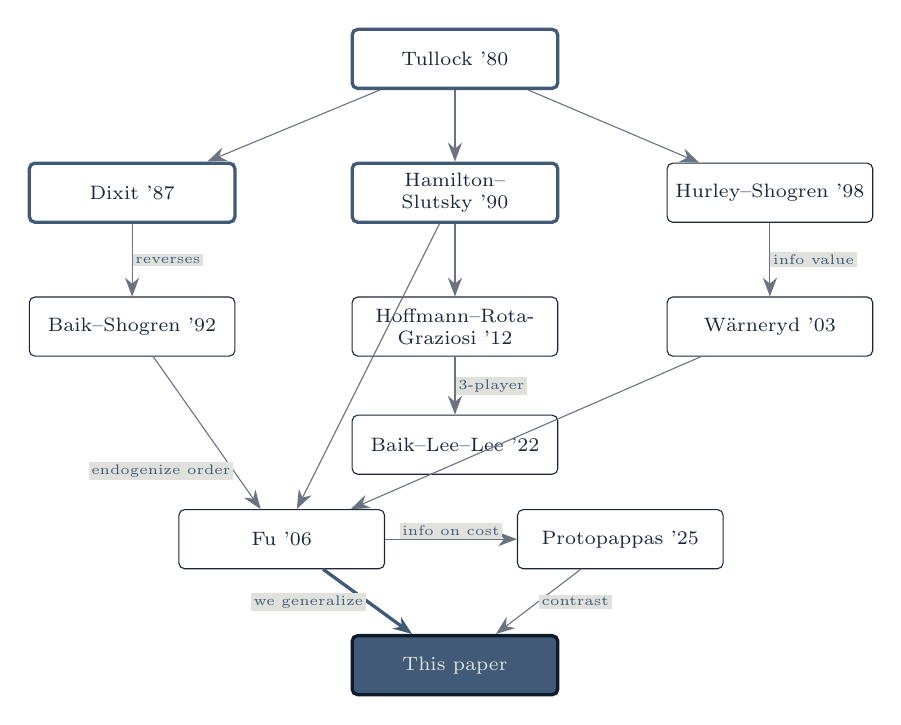
\begin{tikzpicture}[
    >={Stealth[length=2.4mm]},
    font=\scriptsize,
    paper/.style={draw=main, fill=white, rounded corners=2pt,
                  inner sep=3pt, text width=2.4cm, align=center,
                  minimum height=0.75cm, text=main},
    classic/.style={paper, draw=alert, very thick},
    ours/.style={paper, fill=alert, text=background,
                 draw=inkblack, very thick},
    lab/.style={font=\tiny, text=alert, fill=background, inner sep=1pt},
    e/.style={->, draw=main!65},
  ]
    % --- foundation -------------------------------------------------------
    \node[classic] (tul) at (5.5, 0)     {Tullock '80};
    % --- L2: timing in contests ------------------------------------------
    \node[classic] (dix) at (1.4,-1.7)   {Dixit '87};
    \node[paper]   (bs)  at (1.4,-3.4)   {Baik--Shogren '92};
    \node[classic] (hs)  at (5.5,-1.7)   {Hamilton--Slutsky '90};
    \node[paper]   (hof) at (5.5,-3.4)   {Hoffmann--Rota-Graziosi '12};
    \node[paper]   (bll) at (5.5,-4.9)   {Baik--Lee--Lee '22};
    % --- L3: information in contests -------------------------------------
    \node[paper]   (hur) at (9.5,-1.7)   {Hurley--Shogren '98};
    \node[paper]   (war) at (9.5,-3.4)   {W\"arneryd '03};
    % --- confluence ------------------------------------------------------
    \node[paper]   (fu)  at (3.3,-6.1)   {Fu '06};
    \node[paper]   (pro) at (7.6,-6.1)   {Protopappas '25};
    \node[ours]    (us)  at (5.5,-7.7)   {This paper};
    % --- edges -----------------------------------------------------------
    \draw[e] (tul) -- (dix);
    \draw[e] (tul) -- (hs);
    \draw[e] (tul) -- (hur);
    \draw[e] (dix) -- (bs)  node[lab, midway, right]{reverses};
    \draw[e] (hs)  -- (hof);
    \draw[e] (hof) -- (bll) node[lab, midway, right]{3-player};
    \draw[e] (hur) -- (war) node[lab, midway, right]{info value};
    \draw[e] (bs)  -- (fu)  node[lab, near end, left]{endogenize order};
    \draw[e] (hs)  -- (fu);
    \draw[e] (war) -- (fu);
    \draw[e] (fu)  -- (pro) node[lab, midway, above]{info on cost};
    \draw[e, very thick, draw=alert] (fu) -- (us)
          node[lab, midway, left]{we generalize};
    \draw[e] (pro) -- (us) node[lab, midway, right]{contrast};
  \end{tikzpicture}}
  \end{center}
\end{frame}

\begin{frame}{Literature: where we stand}
  \scriptsize
  \setlength{\tabcolsep}{4pt}
  \renewcommand{\arraystretch}{1.15}
  \begin{tabular}{@{}l l l p{3.9cm}@{}}
    \toprule
    \textbf{Paper} & \textbf{Order} & \textbf{Private info} &
    \textbf{Position / how we differ} \\
    \midrule
    \citet{tullock1980}     & ---        & ---        &
      Contest technology; we adopt the $r{=}1$ benchmark \\
    \citet{dixit1987}       & exogenous  & none       &
      Commitment value; we endogenize the order \\
    \citet{baikshogren1992} & endogenous & none       &
      Underdog leads; we add a private value \\
    \citet{hamilton1990}    & endogenous & none       &
      The three-subgame template we reuse \\
    \citet{hoffmann2012}    & endogenous & none       &
      ``Weak leads'' under substitutes; we revise via correlation \\
    \citet{hurley1998}      & exog.\ (sim.) & prize value &
      Effort comparison; we compare \emph{timing} \\
    \citet{warneryd2003}    & exogenous  & common value &
      Info advantage has value; order still fixed \\
    \citet{fu2006}          & endogenous & prize value &
      Signal $\to$ pooling; the perfect-correlation \emph{endpoint} \\
    \citet{protopappas2025} & endogenous & future cost &
      Timing signals cost; we close that channel \\
    \midrule
    \textbf{This paper}     & endogenous & prize value &
      Correlation spectrum; new coexistence region (sep.\ \& pool.) \\
    \bottomrule
  \end{tabular}
\end{frame}

\begin{frame}{Contribution}
  \begin{itemize}
    \item We change \emph{where} the private information sits
    \item Separation becomes a consequence of the \textbf{contest
          structure}, not of a belief assumption or refinement
    \item To our knowledge, this distribution-free form of the
          separation result is new
  \end{itemize}
\end{frame}

% =========================================================================
\section{Model}
% =========================================================================

\begin{frame}{Players \& prize}
  Two risk-neutral players:
  \begin{itemize}
    \item Agent $I$ --- informed
    \item Agent $U$ --- uninformed
  \end{itemize}

  They compete over whether a policy is implemented. Winner takes his
  own prize; loser gets zero.
  \begin{itemize}
    \item $I$ wins $\Rightarrow$ obtains $V_I > 0$
    \item $U$ wins $\Rightarrow$ obtains $V_U \equiv V > 0$
  \end{itemize}
\end{frame}

\begin{frame}{Two layers of asymmetry}
  \begin{itemize}
    \item \textbf{Information}
      \begin{itemize}\normalsize
        \item $U$ knows the prior $G$ of $V_I$, never its realization
        \item $I$ observes $V_I$ privately --- only \emph{after} the
              timing decision
      \end{itemize}
    \item \textbf{Prize}: $I$ receives $V_I$, $U$ receives $V$
          (no requirement $V_I = V$)
  \end{itemize}
\end{frame}

\begin{frame}{Information structure}
  \begin{enumerate}
    \item Stage 0: $I$ and $U$ simultaneously choose \emph{when} to act
          --- $I$ has not yet seen his type
    \item Nature draws $V_I$ from $G$
    \item $I$ observes $V_I$ privately; $U$ does not
    \item Players enter the effort subgame at their committed times
  \end{enumerate}

  \begin{alertblock}{Consequence}
    The stage-0 choice is made on \textbf{ex ante} expected payoffs.
  \end{alertblock}
\end{frame}

\begin{frame}{Timeline of the contest}
\begin{figure}[H]
    \centering
    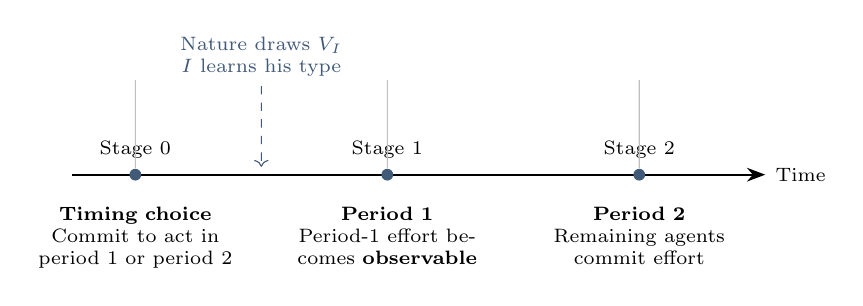
\begin{tikzpicture}[
        xscale=0.8,
        node distance = 1.2cm,
        every node/.style = {font=\scriptsize},
        dot/.style = {circle, fill=black, inner sep=1.5pt}
    ]
    \draw[thick, -{Stealth}] (0,0) -- (11,0) node[right] {Time};

    \node[dot, label=above:{Stage 0}, color=alert] (s0) at (1,0) {};
    \node[dot, label=above:{Stage 1}, color=alert] (s1) at (5,0) {};
    \node[dot, label=above:{Stage 2}, color=alert] (s2) at (9,0) {};

    \node[below=0.2cm of s0, align=center, text width=2.5cm] {
        \textbf{Timing choice}\\
        Commit to act in period 1 or period 2
    };

    \node[align=center, color=alert] (nature) at (3,1.5) {
        Nature draws $V_I$\\
        $I$ learns his type
    };
    \draw[dashed, ->, alert] (nature) -- (3,0.1);

    \node[below=0.2cm of s1, align=center, text width=3cm] {
        \textbf{Period 1}\\
        Period-1 effort becomes \textbf{observable}
    };

    \node[below=0.2cm of s2, align=center, text width=3cm] {
        \textbf{Period 2}\\
        Remaining agents commit effort
    };

    \draw[gray!50, thin] (s0) -- +(0, 1.2);
    \draw[gray!50, thin] (s1) -- +(0, 1.2);
    \draw[gray!50, thin] (s2) -- +(0, 1.2);

    \end{tikzpicture}

    \par\medskip{\footnotesize The three-stage sequential game.\par}
\end{figure}
\end{frame}

\begin{frame}{Three regimes}
  \timinggametable{$\rSS$}{$\rIU$}{$\rUI$}{$\rSS$}

  \vspace{0.5em}
  \begin{itemize}
    \item $\rSS$ --- simultaneous moves
    \item $\rUI$ --- $U$ commits first, $I$ responds
    \item $\rIU$ --- $I$ commits first, $U$ responds
  \end{itemize}
\end{frame}

\begin{frame}{Which regime can carry a signal?}
  \begin{itemize}
    \item $\rSS$ --- simultaneous: no signal
    \item $\rUI$ --- $U$ moves first: no signal from $I$
    \item $\rIU$ --- $I$ moves first, $U$ observes $x_I$:
          \alert{a signal could exist here}
  \end{itemize}

  \vspace{0.5em}
  Only $\rIU$ raises the question of whether $I$'s effort transmits type
  information.
\end{frame}

\begin{frame}{Contest technology}
  Following \citet{tullock1980}, efforts $x_I, x_U \ge 0$ give the
  proportional winning probabilities
  \begin{equation}
    p_I = \dfrac{x_I}{x_I + x_U}, \qquad
    p_U = \dfrac{x_U}{x_I + x_U}.
  \end{equation}
\end{frame}

\begin{frame}{Payoffs}
  Net of effort costs, with $I$ of realized type $v$:
  \begin{align*}
    \pi_I(x_I, x_U; v) &= \dfrac{x_I}{x_I + x_U}\, v - x_I,\\[4pt]
    \pi_U(x_I, x_U; V) &= \dfrac{x_U}{x_I + x_U}\, V - x_U.
  \end{align*}
\end{frame}

\begin{frame}{Best responses}
  Interior first-order conditions give
  \begin{equation}
    x_I^{*}(x_U; v) = \sqrt{v\,x_U} - x_U,
  \end{equation}
  \begin{equation}
    x_U^{*}(x_I; V) = \sqrt{V\,x_I} - x_I.
  \end{equation}

  Outside the interior, the relevant best response is the maximum of
  zero and these expressions.
\end{frame}

\begin{frame}{The crux}
  \begin{alertblock}{The single fact behind every result}
    $x_U^{*}$ depends only on $x_I$ and $V$ --- it contains
    \textbf{no posterior belief} about $V_I$.
  \end{alertblock}

  A signal may exist at the \emph{observational} level, but it never
  enters $U$'s behavior.

  \vspace{0.4em}
  This is the principal departure from \citet{fu2006}.
\end{frame}

\begin{frame}{Stage-0: an ex ante timing game}
  Since $V_I$ is not yet realized, $I$ compares
  $\pt_I^{J} \equiv \E\!\left[\pi_I^{J}(V_I)\right]$,
  $J \in \{\rSS, \rUI, \rIU\}$.

  \timinggametable
    {$(\pt_I^{\rSS},\,\pi_U^{\rSS})$}
    {$(\pt_I^{\rIU},\,\pi_U^{\rIU})$}
    {$(\pt_I^{\rUI},\,\pi_U^{\rUI})$}
    {$(\pt_I^{\rSS},\,\pi_U^{\rSS})$}

  \vspace{0.4em}
  Plan: solve the three effort subgames, then read this $2\times 2$ game.
\end{frame}

% =========================================================================
\section{Equilibrium Analysis}
% =========================================================================

\begin{frame}{Notation: moments of the prior}
  \begin{equation}
    \mu \equiv \E[V_I], \quad
    \kappa \equiv \E\!\Big[\dfrac{1}{\sqrt{V_I}}\Big], \quad
    \nu \equiv \E[\sqrt{V_I}], \quad
    \lambda \equiv \E\!\Big[\dfrac{1}{V_I}\Big].
  \end{equation}

  \begin{itemize}
    \item All assumed finite; each subgame has an interior solution
    \item What matters: how timing reorders \textbf{commitment},
          \textbf{observation}, \textbf{response}
  \end{itemize}
\end{frame}

\begin{frame}{$\rSS$: simultaneous --- efforts}
  $I$ tailors effort to type; $U$ chooses one effort under uncertainty.
  \begin{equation}
    x_U^{\rSS} = \dfrac{V^2\kappa^2}{(1+V\lambda)^2},
  \end{equation}
  \begin{equation}
    x_I^{\rSS}(v) = \dfrac{V\kappa\sqrt{v}}{1+V\lambda} - x_U^{\rSS}.
  \end{equation}

  \alert{Simultaneity $\neq$ symmetric effort.}
\end{frame}

\begin{frame}{$\rSS$: ex ante payoffs}
  \begin{equation*}
    \pt_I^{\rSS} = \mu - \dfrac{2V\kappa\nu}{1+V\lambda}
      + \dfrac{V^2\kappa^2}{(1+V\lambda)^2},
  \end{equation*}
  \begin{equation*}
    \pi_U^{\rSS} = \dfrac{V^3\kappa^2\lambda}{(1+V\lambda)^2}.
  \end{equation*}

  $U$'s effort absorbs the ex ante uncertainty about $I$'s type.

  \begin{proof}
    \hyperref[prf:ss]{See proof in page \pageref{prf:ss}.}
  \end{proof}
\end{frame}

\begin{frame}{$\rUI$: uninformed leader --- efforts}
  $U$ commits first; $I$ responds type-by-type.
  \begin{equation}
    x_U^{\rUI} = \dfrac{V^2\kappa^2}{4},
  \end{equation}
  \begin{equation}
    x_I^{\rUI}(v) = \dfrac{V\kappa\sqrt{v}}{2} - \dfrac{V^2\kappa^2}{4}.
  \end{equation}

  $U$'s effort is now a \textbf{Stackelberg commitment}, not the
  simultaneous FOC.
\end{frame}

\begin{frame}{$\rUI$: ex ante payoffs}
  \begin{equation*}
    \pt_I^{\rUI} = \mu - V\kappa\nu + \dfrac{V^2\kappa^2}{4},
  \end{equation*}
  \begin{equation*}
    \pi_U^{\rUI} = \dfrac{V^2\kappa^2}{4}.
  \end{equation*}

  \begin{proof}
    \hyperref[prf:ui]{See proof in page \pageref{prf:ui}.}
  \end{proof}
\end{frame}

\begin{frame}{$\rIU$: informed leader --- efforts}
  $I$ moves first; $U$ responds to $x_I$ --- but his best response
  ignores beliefs.
  \begin{equation}
    x_I^{\rIU}(v) = \dfrac{v^2}{4V},
    \qquad
    x_U^{\rIU}(v) = \dfrac{v(2V-v)}{4V}.
  \end{equation}
  \begin{equation*}
    \pt_I^{\rIU} = \dfrac{\E[V_I^2]}{4V}.
  \end{equation*}
\end{frame}

\begin{frame}{$\rIU$: the separation theorem}
  \begin{theorem}[Unique separating equilibrium]
    If type $v$ mimics any $s \neq v$, the payoff loss is
    \begin{equation*}
      \dfrac{(v-s)^2}{4V} > 0.
    \end{equation*}
  \end{theorem}

  Every type strictly prefers its own action $\Rightarrow$ pooling and
  semi-separating equilibria are ruled out. \alert{Distribution-free.}

  \begin{proof}
    \hyperref[prf:iu]{See proof in page \pageref{prf:iu}.}
  \end{proof}
\end{frame}

\begin{frame}{Three regimes side by side}
  \small
  \begin{table}[H]
    \centering
    \renewcommand{\arraystretch}{1.6}
    \begin{tabular}{lcc}
      \toprule
      & $\pt_I^{J}$ & $\pi_U^{J}$\\
      \midrule
      $\rSS$ & $\mu - \frac{2V\kappa\nu}{1+V\lambda}
               + \frac{V^2\kappa^2}{(1+V\lambda)^2}$
             & $\frac{V^3\kappa^2\lambda}{(1+V\lambda)^2}$\\
      $\rUI$ & $\mu - V\kappa\nu + \frac{V^2\kappa^2}{4}$
             & $\frac{V^2\kappa^2}{4}$\\
      $\rIU$ & $\frac{\E[V_I^2]}{4V}$
             & $\frac{4V^2 - 4V\mu + \E[V_I^2]}{4V}$\\
      \bottomrule
    \end{tabular}
  \end{table}

  These feed directly into the stage-0 game.
\end{frame}

% =========================================================================
\section{Endogenous Timing}
% =========================================================================

\begin{frame}{Back to the stage-0 game}
  \timinggametable
    {$(\pt_I^{\rSS},\,\pi_U^{\rSS})$}
    {$(\pt_I^{\rIU},\,\pi_U^{\rIU})$}
    {$(\pt_I^{\rUI},\,\pi_U^{\rUI})$}
    {$(\pt_I^{\rSS},\,\pi_U^{\rSS})$}

  We compare unilateral deviations from this timing game.
\end{frame}

\begin{frame}{Four deviation differences}
  \begin{align*}
    \Delta_I^{\rUI} &\equiv \pt_I^{\rUI} - \pt_I^{\rSS}, &
    \Delta_I^{\rIU} &\equiv \pt_I^{\rIU} - \pt_I^{\rSS},\\[4pt]
    \Delta_U^{\rSS} &\equiv \pi_U^{\rSS} - \pi_U^{\rIU}, &
    \Delta_U^{\rUI} &\equiv \pi_U^{\rUI} - \pi_U^{\rSS}.
  \end{align*}

  Each sign tells us whether a player wants to deviate from a candidate
  profile.
\end{frame}

\begin{frame}{The key asymmetry}
  \begin{alertblock}{$U$'s deviation when $I$ moves second}
    \begin{equation*}
      \Delta_U^{\rUI}
      = \dfrac{V^2\kappa^2 (1-V\lambda)^2}{4(1+V\lambda)^2}
      \;\ge\; 0.
    \end{equation*}
  \end{alertblock}

  Whenever $I$ plans to move second, $U$ generically prefers to move
  first --- equality only at the knife-edge $V\lambda = 1$.
\end{frame}

\begin{frame}{Stage-0 best responses (Lemma)}
  \begin{lemma}[Best responses in the stage-0 timing game]
    \begin{itemize}
      \item If $U$ chooses period 1, then $I$ chooses period 2 iff
            $\Delta_I^{\rUI} > 0$; otherwise he chooses period 1.
      \item If $U$ chooses period 2, then $I$ chooses period 1 iff
            $\Delta_I^{\rIU} > 0$; otherwise he chooses period 2.
      \item If $I$ chooses period 1, then $U$ chooses period 1 iff
            $\Delta_U^{\rSS} > 0$; otherwise he chooses period 2.
      \item If $I$ chooses period 2, then $U$ weakly prefers period 1
            because $\Delta_U^{\rUI} \ge 0$.
    \end{itemize}
  \end{lemma}

  \begin{proof}
    \hyperref[prf:br]{See proof in page \pageref{prf:br}.}
  \end{proof}
\end{frame}

\begin{frame}{Which regimes are equilibria?}
  \begin{theorem}[Pure-strategy timing equilibria]
    \begin{itemize}
      \item $\rUI$ \;$\Leftrightarrow$\; $\Delta_I^{\rUI} \ge 0$
      \item Immediate $\rSS$ \;$\Leftrightarrow$\;
            $\Delta_I^{\rUI} \le 0$ and $\Delta_U^{\rSS} \ge 0$
      \item $\rIU$ \;$\Leftrightarrow$\;
            $\Delta_I^{\rIU} \ge 0$ and $\Delta_U^{\rSS} \le 0$
      \item Delayed $\rSS$ \;$\Leftrightarrow$\;
            $\Delta_I^{\rIU} \le 0$ and $V\lambda = 1$
    \end{itemize}
  \end{theorem}

  \begin{proof}
    \hyperref[prf:timing]{See proof in page \pageref{prf:timing}.}
  \end{proof}
\end{frame}

\begin{frame}{No refinement needed}
  \begin{itemize}
    \item Regime selection is read \textbf{directly} from the four
          deviation differences
    \item Delayed $\rSS$ needs the knife-edge $V\lambda = 1$
    \item For generic parameters it cannot be a pure-strategy
          equilibrium
  \end{itemize}
\end{frame}

\begin{frame}{Why ex ante, not type-level}
  Define the ex post comparison for a realized type:
  \begin{equation}
    R(v) \equiv \pi_I^{\rSS}(v) - \pi_I^{\rIU}(v)
    = \Big(\sqrt{v} - \dfrac{V\kappa}{1+V\lambda}\Big)^2
      - \dfrac{v^2}{4V}.
  \end{equation}
\end{frame}

\begin{frame}{The decision rule}
  \begin{alertblock}{Identity}
    \begin{equation*}
      \E[R(V_I)] = \pt_I^{\rSS} - \pt_I^{\rIU}
      = -\,\Delta_I^{\rIU}.
    \end{equation*}
  \end{alertblock}

  A single type's ex post preference is just a \textbf{decomposition};
  the stage-0 choice is governed by the \emph{average}.

  \begin{proof}
    \hyperref[prf:rv]{See proof in page \pageref{prf:rv}.}
  \end{proof}
\end{frame}

\begin{frame}{Two-point distribution (Lemma)}
  \begin{lemma}[Two-point sign test]
    Let $V_I \in \{v_L, v_H\}$. Comparing the signs of $R(v_L)$ and
    $R(v_H)$ gives:
    \begin{itemize}
      \item $(-,-)$: both types prefer moving first, so
            $\Delta_I^{\rIU} > 0$
      \item $(+,+)$: both types prefer moving second, so
            $\Delta_I^{\rIU} < 0$
      \item mixed signs: the aggregate sign is determined by the
            probability-weighted average
    \end{itemize}
  \end{lemma}

  \begin{proof}
    \hyperref[prf:two-point]{See proof in page \pageref{prf:two-point}.}
  \end{proof}
\end{frame}

\begin{frame}{Two-point: timing regions}
  \begin{figure}[H]
    \centering
    
\includegraphics[width=0.9\textwidth]{fig5_regions.pdf}

    \par\medskip{\footnotesize Sign regions on the $(\mu,\delta)$ plane.\par}
  \end{figure}

  \centering
  \small $V$, $\mu$, $\delta$ \emph{jointly} set the timing preference.
\end{frame}

\begin{frame}{Uniform distribution (Lemma)}
  \begin{lemma}[Uniform threshold characterization]
    If $V_I \sim \mathcal{U}[\mu-\delta,\,\mu+\delta]$, then the
    continuity of $R(v)$ implies:
    \begin{itemize}
      \item opposite endpoint signs $\Rightarrow$ an interior threshold
            $v^{*}$ where the comparison reverses
      \item same endpoint sign $\Rightarrow$ all types prefer the same
            direction
    \end{itemize}
  \end{lemma}

  \begin{proof}
    \hyperref[prf:uniform]{See proof in page \pageref{prf:uniform}.}
  \end{proof}
\end{frame}

\begin{frame}{Uniform: timing regions}
  \begin{figure}[H]
    \centering
    
\includegraphics[width=0.9\textwidth]{fig5_uniform_regions.pdf}

    \par\medskip{\footnotesize Type-partition regions; panels are $V=0.5$, $1.0$, and $1.5$.\par}
  \end{figure}

  \centering
  \small As $V$ rises, the split region expands.
\end{frame}

\begin{frame}{Welfare $\neq$ equilibrium ranking}
  Total expected welfare $\E[W] = \pt_I + \pi_U$:
  \begin{align*}
    \E[W^{\rUI}] &= \mu - V\kappa\nu + \dfrac{1}{2}V^2\kappa^2,\\[3pt]
    \E[W^{\rIU}] &= V - \mu + \dfrac{\E[V_I^2]}{2V}.
  \end{align*}

  Equilibrium checks \emph{unilateral deviations}; welfare
  \emph{aggregates}. No fixed monotone correspondence.

  \begin{proof}
    \hyperref[prf:welfare]{See proof in page \pageref{prf:welfare}.}
  \end{proof}
\end{frame}

% =========================================================================
\section{Extension: Partially Correlated Types}
% =========================================================================

\begin{frame}{Relaxing the key assumption}
  The unique separating equilibrium relied on $U$'s prize being a known
  constant $V$.

  \begin{block}{Now}
    Let $U$'s prize also be random, $V_U \in \{V_L, V_H\}$, and
    \textbf{positively correlated} with $V_I$ via a single parameter
    $\rho \in [0,1]$.
  \end{block}
\end{frame}

\begin{frame}{Partial correlation structure}
  Single parameter $\rho \in [0,1]$: Pearson correlation between $V_I$ and $V_U$.

  Diagonal mass of the joint distribution:
  \begin{equation}
    \Pr(V_I=V_H, V_U=V_H) = q^2 + \rho\,q(1-q).
  \end{equation}

  Conditional probabilities are clean linear functions of $\rho$:
  \begin{align*}
    p_H &\equiv \Pr(V_U=V_H \mid V_I=V_H) = q + \rho(1-q),\\
    p_L &\equiv \Pr(V_U=V_L \mid V_I=V_L) = 1 - q(1-\rho).
  \end{align*}
\end{frame}

\begin{frame}{Three benchmarks}
  \begin{itemize}
    \item $\rho = 0$: statistical independence ---
          the baseline model ($V_U \equiv V$)
    \item $\rho = 1$: full correlation ---
          exactly \citet{fu2006}
    \item $0 < \rho < 1$: partial correlation --- the focus of this
          chapter
  \end{itemize}
\end{frame}

\begin{frame}{Belief-weighted prize}
  $U$'s effective prize is no longer constant.
  With posterior $m = \Pr(V_I=V_H \mid x_I)$:
  \begin{equation}
    \Vhat(m) = V_L + \bigl[q + \rho(m-q)\bigr]\Delta V,
    \qquad \Delta V = V_H - V_L.
  \end{equation}

  \vspace{0.3em}
  Key: $\Vhat(q) = qV_H + (1-q)V_L$ is \emph{independent of $\rho$} ---
  the $\rSS$ payoffs are unaffected by correlation.
\end{frame}

\begin{frame}{Sensitivity to beliefs}
  \begin{equation}
    \dfrac{d\Vhat}{dm} = \rho\,\Delta V.
  \end{equation}

  \begin{itemize}
    \item $\rho = 0$: derivative $= 0$ --- beliefs carry no value
    \item $\rho > 0$: a higher posterior raises $U$'s expected own prize
          proportionally to $\rho$
  \end{itemize}
\end{frame}

\begin{frame}{Dual inference}
  \begin{alertblock}{Mechanism}
    A high-effort signal means a \textbf{stronger opponent}
    \emph{and} a \textbf{higher own prize}.
  \end{alertblock}

  The ``higher stakes'' effect offsets deterrence: under positive
  correlation, $x_U^{*}$ is \textbf{increasing} in $m$. $U$ no longer
  retreats from a high signal.
\end{frame}

\begin{frame}{A numerical illustration}
  Fix $V_H=2$, $V_L=1$, $q=0.5$, observed $x_I=1$.
  \begin{itemize}
    \item Independence ($\rho=0$): $\Vhat\equiv 1.5$,
          $x_U^{*}=\sqrt{1.5}-1\approx 0.225$
    \item Positive corr.\ ($\rho=0.6$): $\Vhat(0)=1.2$, $\Vhat(1)=1.8$;
          $x_U^{*}$ runs $0.095 \to 0.342$ --- more than tripling
  \end{itemize}
\end{frame}

\begin{frame}{When does separation survive?}
  Only the high type's incentive constraint binds:
  \begin{equation}
    \dfrac{\Vhat(1)}{\Vhat(0)} \;\le\; R
    \equiv \dfrac{V_H^2}{V_L(2V_H - V_L)}.
  \end{equation}

  The low type never gains from upward mimicry --- its constraint holds
  automatically.
\end{frame}

\begin{frame}{The critical correlation $\rho^{*}$}
  Because $\Vhat(1)/\Vhat(0)$ is strictly increasing in $\rho$, the
  separation condition translates to a unique critical value:
  \begin{equation}
    \rho^{*}
    = \dfrac{(R-1)\,\Vhat(q)}{\Delta V\,(1-q+Rq)},
    \qquad
    R = \dfrac{V_H^2}{V_L(2V_H-V_L)}.
  \end{equation}

  Undistorted separation holds iff $\rho \le \rho^{*}$.

  \begin{proof}
    \hyperref[prf:ch6]{See proof in page \pageref{prf:ch6}.}
  \end{proof}
\end{frame}

\begin{frame}{Riley distorted separation ($\rho > \rho^{*}$)}
  When $\rho > \rho^{*}$, undistorted separation fails.
  But low type can \textbf{distort effort downward} to block mimicry.

  \begin{block}{D1 refinement selects the unique distorted equilibrium}
    \begin{equation*}
      x_L^{\mathrm{Riley}} = (z_H^{-})^2
      = \dfrac{V_H^2}{4\Vhat(0)}\bigl(1-\sqrt{\alpha_{\mathrm{sep}}}\bigr)^2,
      \quad
      \alpha_{\mathrm{sep}} \equiv 1 - \dfrac{\Vhat(0)}{\Vhat(1)}.
    \end{equation*}
    This is the minimum-cost separating equilibrium (\citet{riley1979}).
  \end{block}

  At baseline $V_H = 2V_L$: Riley distorted separation coexists with
  pooling for \emph{all} $\rho \in (\rho^{*}, 1]$.
\end{frame}

\begin{frame}{Pooling steps in}
  When separation collapses, a pooling equilibrium also supports play.
  With $\alpha \equiv 1 - \Vhat(q)/\Vhat(1)$, it exists iff
  \begin{equation}
    \sqrt{\alpha} \;\ge\; \dfrac{V_H - V_L}{V_H + V_L}.
  \end{equation}

  Pooling appears at $\rho = \rho_P < \rho^{*}$.
  At $\rho = 0$: $\alpha = 0$ --- no pooling, consistent with
  unique separation at independence.
\end{frame}

\begin{frame}{Four equilibrium regions}
  \begin{figure}[H]
    \centering
    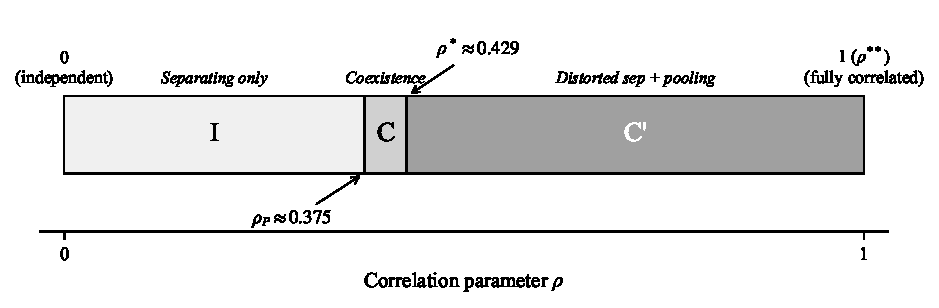
\includegraphics[width=0.9\textwidth]{fig6_pooling_regions.pdf}

    \par\medskip{\footnotesize Equilibrium regions along the $\rho \in [0,1]$ spectrum.\par}
  \end{figure}

  \centering
  \small
  \textbf{I}: sep.\ only \quad
  \textbf{C}: undist.\ sep.+pool.\ \quad
  \textbf{C'}: Riley+pool.\ \quad
  \textbf{II}: pool.\ only (empty at $V_H=2V_L$)
\end{frame}

\begin{frame}{One continuous spectrum}
  \begin{figure}[H]
    \centering
    
\includegraphics[width=0.72\textwidth]{fig6_spectrum.pdf}

    \par\medskip{\footnotesize Effective prize ratio $\Vhat(1)/\Vhat(0)$ crosses $R$ uniquely at $\rho^{*}$.\par}
  \end{figure}

  \centering
  \small Along the $\rho$-axis the ratio rises monotonically from
  $1$ (at $\rho=0$) to $V_H/V_L$ (at $\rho=1$).
\end{frame}

\begin{frame}{Timing preference reversal}
  \begin{alertblock}{Proposition}
    For $\rho \in [0, \rho^{*}]$, $I$'s gain from moving first,
    $\Delta_I^{\rIU}(\rho)$, is \textbf{strictly decreasing} in $\rho$.
  \end{alertblock}
  \begin{itemize}
    \item $\rho=0$: baseline --- $I$ may prefer to move first
    \item $\rho=1$: exactly \citet{fu2006} --- $I$ strictly prefers to wait
    \item Unique crossing $\rho^{\dagger} \in (0,1]$
  \end{itemize}

  \vspace{0.3em}
  Fu's ``informed player always waits'' is the $\rho=1$ endpoint of this
  spectrum.
\end{frame}

\begin{frame}{Unifying message}
  \begin{alertblock}{Spectrum}
    Baseline and \citet{fu2006} are the \textbf{two endpoints} of one
    correlation spectrum.
  \end{alertblock}

  Fu's pooling outcome is the \emph{degenerate extreme} of the present
  framework, not a separate world.
\end{frame}

% =========================================================================
\section{Conclusion}
% =========================================================================

\begin{frame}{What we showed}
  \begin{itemize}
    \item Relocating the private information closes the signal at the
          effort level
    \item The $\rIU$ separating equilibrium is then
          \alert{distribution-free}
    \item Timing is an \textbf{ex ante} payoff comparison;
          $V,\mu,\delta$ act jointly
    \item Correlation rebuilds a smooth separating $\to$ pooling
          spectrum
  \end{itemize}
\end{frame}

\begin{frame}{Takeaway}
  \begin{block}{}
    Whether separation holds is about \emph{where} private information
    sits --- not about belief refinements.
  \end{block}
\end{frame}

\begin{frame}[focus]
  Thank you.

  \vspace{0.5em}
  \small Questions \& discussion
\end{frame}

\begin{frame}[allowframebreaks]{References}
  \bibliographystyle{apalike}
  {
    \renewcommand{\bibsection}{\vspace{-5pt}}
    \bibliography{demo}
  }
\end{frame}

% =========================================================================
\appendix
% =========================================================================

\begin{frame}[focus]
  Appendix: Proofs
\end{frame}

\begin{frame}[allowframebreaks]{$\rSS$ subgame}\label{prf:ss}
  \begin{proof}
    For type $v$, $I$'s best response to $x_U$ is
    \[
      x_I(v) = \sqrt{v\,x_U} - x_U .
    \]
    Anticipating this type-contingent response, $U$ chooses $x_U$ from
    the first-order condition
    \[
      V \,\E\!\left[ \dfrac{x_I(V_I)}{\left(x_I(V_I)+x_U\right)^2} \right]
      = 1 .
    \]
    Since $x_I(v)+x_U = \sqrt{v\,x_U}$, the bracket simplifies and
    \[
      V \,\E\!\left[ \dfrac{\sqrt{V_I x_U}-x_U}{V_I x_U} \right]
      = V\!\left( \dfrac{\kappa}{\sqrt{x_U}} - \lambda \right) = 1 ,
    \]
    hence
    \[
      \sqrt{x_U^{\rSS}} = \dfrac{V\kappa}{1+V\lambda},
      \qquad
      x_U^{\rSS} = \dfrac{V^2\kappa^2}{\left(1+V\lambda\right)^2}.
    \]
    Substituting back,
    \[
      x_I^{\rSS}(v)
      = \dfrac{V\kappa\sqrt{v}}{1+V\lambda}
        - \dfrac{V^2\kappa^2}{\left(1+V\lambda\right)^2}.
    \]
    Because $x_I^{\rSS}(v)+x_U^{\rSS} = \frac{V\kappa\sqrt{v}}{1+V\lambda}$,
    \begin{align*}
      \pi_I^{\rSS}(v)
        &= \left(1 - \dfrac{V\kappa}{(1+V\lambda)\sqrt{v}}\right) v
           - x_I^{\rSS}(v)
         = \left( \sqrt{v} - \dfrac{V\kappa}{1+V\lambda} \right)^{2}, \\[4pt]
      \pi_U^{\rSS}(v)
        &= \dfrac{V^2\kappa}{(1+V\lambda)\sqrt{v}}
           - \dfrac{V^2\kappa^2}{\left(1+V\lambda\right)^2}.
    \end{align*}
    Taking expectations over $V_I$ gives the ex ante payoffs
    \begin{align*}
      \pt_I^{\rSS}
        &= \mu - \dfrac{2V\kappa\nu}{1+V\lambda}
           + \dfrac{V^2\kappa^2}{\left(1+V\lambda\right)^2}, \\[4pt]
      \pi_U^{\rSS}
        &= \dfrac{V^2\kappa}{1+V\lambda}\,\kappa
           - \dfrac{V^2\kappa^2}{\left(1+V\lambda\right)^2}
         = \dfrac{V^3\kappa^2\lambda}{\left(1+V\lambda\right)^2}.
    \end{align*}
  \end{proof}
\end{frame}

\begin{frame}[allowframebreaks]{$\rUI$ subgame}\label{prf:ui}
  \begin{proof}
    Given $x_U$ and type $v$, $I$'s best response is
    $x_I(v) = \sqrt{v\,x_U} - x_U$. Committing first, $U$ solves
    \[
      \max_{x_U\ge 0}\;
      \E\!\left[ V\sqrt{\dfrac{x_U}{V_I}} - x_U \right]
      = \max_{x_U\ge 0}\; \left( V\sqrt{x_U}\,\kappa - x_U \right).
    \]
    The first-order condition $\frac{V\kappa}{2\sqrt{x_U}} - 1 = 0$
    yields
    \[
      x_U^{\rUI} = \dfrac{V^2\kappa^2}{4},
      \qquad
      x_I^{\rUI}(v) = \dfrac{V\kappa\sqrt{v}}{2}
                      - \dfrac{V^2\kappa^2}{4}.
    \]
    Since $x_I^{\rUI}(v)+x_U^{\rUI} = \frac{V\kappa\sqrt{v}}{2}$,
    \[
      \pi_I^{\rUI}(v) = \left( \sqrt{v} - \dfrac{V\kappa}{2} \right)^{2},
      \qquad
      \pi_U^{\rUI}(v) = \dfrac{V^2\kappa}{2\sqrt{v}}
                        - \dfrac{V^2\kappa^2}{4}.
    \]
    Taking expectations,
    \[
      \pt_I^{\rUI} = \mu - V\kappa\nu + \dfrac{V^2\kappa^2}{4},
      \qquad
      \pi_U^{\rUI} = \dfrac{V^2\kappa}{2}\,\kappa
                     - \dfrac{V^2\kappa^2}{4}
                   = \dfrac{V^2\kappa^2}{4}.
    \]
  \end{proof}
\end{frame}

\begin{frame}[allowframebreaks]{$\rIU$ subgame}\label{prf:iu}
  \begin{proof}
    Given $x_I$, $U$'s best response is
    $x_U^{*}(x_I;V) = \sqrt{V x_I} - x_I$. Anticipating it, type $v$
    maximizes
    \[
      W(x_I;v)
      = \dfrac{x_I}{x_I + x_U^{*}(x_I;V)}\, v - x_I
      = \dfrac{v}{\sqrt{V}}\sqrt{x_I} - x_I ,
    \]
    which is strictly concave. The first-order condition
    $\frac{v}{2\sqrt{V x_I}} - 1 = 0$ gives
    \[
      x_I^{\rIU}(v) = \dfrac{v^2}{4V},
      \qquad
      x_U^{\rIU}(v)
      = \sqrt{V\,\dfrac{v^2}{4V}} - \dfrac{v^2}{4V}
      = \dfrac{v\left(2V-v\right)}{4V}.
    \]
    Hence
    \[
      \pi_I^{\rIU}(v) = \dfrac{v^2}{4V},
      \qquad
      \pi_U^{\rIU}(v) = \dfrac{\left(2V-v\right)^2}{4V},
    \]
    and, in expectation,
    \[
      \pt_I^{\rIU} = \dfrac{\E\!\left[V_I^2\right]}{4V},
      \qquad
      \pi_U^{\rIU}
      = \dfrac{4V^2 - 4V\mu + \E\!\left[V_I^2\right]}{4V}.
    \]
    \emph{Incentive compatibility.} If type $v$ mimics any $s\neq v$ it
    exerts $s^2/(4V)$; after $U$'s response the deviation payoff is
    \[
      \widetilde{U}(v,s)
      = \dfrac{v}{\sqrt{V}}\sqrt{\dfrac{s^2}{4V}} - \dfrac{s^2}{4V}
      = \dfrac{2vs - s^2}{4V}.
    \]
    The truthful payoff is $v^2/(4V)$, so
    \[
      \dfrac{v^2}{4V} - \widetilde{U}(v,s)
      = \dfrac{\left(v-s\right)^2}{4V} > 0
      \qquad (s\neq v).
    \]
    Every type strictly prefers its own action; pooling and
    semi-separating profiles violate incentive compatibility, so the
    perfect Bayesian equilibrium of the $\rIU$ subgame is the unique
    separating one.
  \end{proof}
\end{frame}

\begin{frame}[allowframebreaks]{Ex post decomposition $R(v)$}\label{prf:rv}
  \begin{proof}
    By definition,
    \[
      R(v) = \pi_I^{\rSS}(v) - \pi_I^{\rIU}(v)
           = \left( \sqrt{v} - \dfrac{V\kappa}{1+V\lambda} \right)^{2}
             - \dfrac{v^2}{4V}.
    \]
    Taking expectations over $V_I$,
    \[
      \E\!\left[R(V_I)\right]
      = \pt_I^{\rSS} - \pt_I^{\rIU}
      = -\,\Delta_I^{\rIU}.
    \]
    Next, $R(v)\le 0$ is equivalent to
    \[
      \left( \sqrt{v} - \dfrac{V\kappa}{1+V\lambda} \right)^{2}
      \le \dfrac{v^2}{4V}
      \iff
      \left| \sqrt{v} - \dfrac{V\kappa}{1+V\lambda} \right|
      \le \dfrac{v}{2\sqrt{V}} .
    \]
    Since $v/(2\sqrt{V})>0$, this absolute-value inequality rewrites as
    \[
      \dfrac{V\kappa}{1+V\lambda}
      \in
      \left[\, \sqrt{v} - \dfrac{v}{2\sqrt{V}},\;
               \sqrt{v} + \dfrac{v}{2\sqrt{V}} \,\right].
    \]
    For two-point support, compare the signs of $R(v_L)$ and $R(v_H)$.
    For the uniform case, continuity and the intermediate value theorem
    yield an interior root that partitions the support.
  \end{proof}
\end{frame}

\begin{frame}{Stage-0 best responses}\label{prf:br}
  \begin{proof}
    Fix the opponent's timing choice and compare the two cells in the
    stage-0 payoff table. If $U$ chooses period 1, then $I$ compares
    $\pt_I^{\rUI}$ against $\pt_I^{\rSS}$, so period 2 is optimal iff
    $\Delta_I^{\rUI} = \pt_I^{\rUI} - \pt_I^{\rSS} > 0$. If $U$ chooses
    period 2, then $I$ compares $\pt_I^{\rIU}$ against $\pt_I^{\rSS}$,
    so period 1 is optimal iff $\Delta_I^{\rIU} > 0$.

    Symmetrically, if $I$ chooses period 1, then $U$ compares
    $\pi_U^{\rSS}$ against $\pi_U^{\rIU}$, so period 1 is optimal iff
    $\Delta_U^{\rSS} = \pi_U^{\rSS} - \pi_U^{\rIU} > 0$. If $I$ chooses
    period 2, then $U$ compares $\pi_U^{\rUI}$ against $\pi_U^{\rSS}$,
    and period 1 is weakly optimal exactly when
    $\Delta_U^{\rUI} \ge 0$.
  \end{proof}
\end{frame}

\begin{frame}[allowframebreaks]{Pure-strategy timing equilibria}\label{prf:timing}
  \begin{proof}
    A pure-strategy equilibrium is a cell in the stage-0 timing game in
    which both players best respond.

    \begin{itemize}
      \item $\rUI$: by the best-response lemma, this cell is an
            equilibrium exactly when $I$ weakly prefers period 2 after
            $U$ chooses period 1, i.e. when $\Delta_I^{\rUI} \ge 0$.
      \item Immediate $\rSS$: this requires that $I$ does not deviate
            to period 2 when $U$ chooses period 1 and that $U$ does not
            deviate to period 2 when $I$ chooses period 1, so
            $\Delta_I^{\rUI} \le 0$ and $\Delta_U^{\rSS} \ge 0$.
      \item $\rIU$: this requires that $I$ weakly prefers period 1 when
            $U$ chooses period 2 and that $U$ weakly prefers period 2
            when $I$ chooses period 1, hence $\Delta_I^{\rIU} \ge 0$
            and $\Delta_U^{\rSS} \le 0$.
      \item Delayed $\rSS$: this requires
            $\Delta_I^{\rIU} \le 0$ and $\Delta_U^{\rUI} \le 0$. Since
            $\Delta_U^{\rUI} \ge 0$ always, the latter holds iff
            $\Delta_U^{\rUI} = 0$, i.e. iff $V\lambda = 1$.
    \end{itemize}
  \end{proof}
\end{frame}

\begin{frame}{Two-point sign test}\label{prf:two-point}
  \begin{proof}
    When $V_I$ has support $\{v_L,v_H\}$ with probabilities
    $1-q$ and $q$,
    \[
      \E[R(V_I)] = (1-q)R(v_L) + qR(v_H).
    \]
    Since $\E[R(V_I)] = -\,\Delta_I^{\rIU}$ by
    \hyperref[prf:rv]{the decomposition proof}, if both endpoint values
    are negative then $\E[R(V_I)] < 0$ and thus $\Delta_I^{\rIU} > 0$.
    If both are positive then $\E[R(V_I)] > 0$ and
    $\Delta_I^{\rIU} < 0$.

    If the endpoint signs differ, then the sign of $\E[R(V_I)]$ is not
    pinned down pointwise; it is determined by the probability-weighted
    average of the two endpoint values.
  \end{proof}
\end{frame}

\begin{frame}{Uniform threshold characterization}\label{prf:uniform}
  \begin{proof}
    Under $V_I \sim \mathcal{U}[\mu-\delta,\,\mu+\delta]$, the function
    $R(v)$ is continuous on the compact support. If the endpoint values
    have opposite signs, the intermediate value theorem implies the
    existence of some $v^{*} \in (\mu-\delta,\mu+\delta)$ such that
    $R(v^{*}) = 0$, so preferences reverse at an interior threshold.

    If both endpoints have the same sign, continuity rules out any sign
    change on the interval, and all types therefore prefer the same
    timing direction.
  \end{proof}
\end{frame}

\begin{frame}{Welfare expressions}\label{prf:welfare}
  \begin{proof}
    Total expected welfare in regime $J$ is
    $\E[W^{J}] = \pt_I^{J} + \pi_U^{J}$. Summing the ex ante payoffs,
    \begin{align*}
      \E\!\left[W^{\rSS}\right]
        &= \pt_I^{\rSS} + \pi_U^{\rSS} \\
        &= \mu - \dfrac{2V\kappa\nu}{1+V\lambda}
           + \dfrac{V^2\kappa^2}{\left(1+V\lambda\right)^2}
           + \dfrac{V^3\kappa^2\lambda}{\left(1+V\lambda\right)^2}, \\[6pt]
      \E\!\left[W^{\rUI}\right]
        &= \pt_I^{\rUI} + \pi_U^{\rUI}
         = \left( \mu - V\kappa\nu + \dfrac{V^2\kappa^2}{4} \right)
           + \dfrac{V^2\kappa^2}{4} \\
        &= \mu - V\kappa\nu + \dfrac{1}{2}V^2\kappa^2, \\[6pt]
      \E\!\left[W^{\rIU}\right]
        &= \pt_I^{\rIU} + \pi_U^{\rIU}
         = \dfrac{\E\!\left[V_I^2\right]}{4V}
           + \dfrac{4V^2 - 4V\mu + \E\!\left[V_I^2\right]}{4V} \\
        &= V - \mu + \dfrac{\E\!\left[V_I^2\right]}{2V}.
    \end{align*}
  \end{proof}
\end{frame}

\begin{frame}[allowframebreaks]{Critical correlation $\rho^{*}$}\label{prf:ch6}
  \begin{proof}
    Set the high-type IC with equality:
    $\Vhat(1)/\Vhat(0) = R$, where
    $R = V_H^2/[V_L(2V_H-V_L)]$.
    Substituting
    \[
      \Vhat(1) = V_L + [q+\rho(1-q)]\Delta V,
      \qquad
      \Vhat(0) = V_L + q(1-\rho)\Delta V,
    \]
    the equality $\Vhat(1) = R\,\Vhat(0)$ expands to
    \[
      V_L + [q+\rho(1-q)]\Delta V
      = R\bigl(V_L + q(1-\rho)\Delta V\bigr).
    \]
    Collecting $\rho$ terms:
    \[
      \rho\bigl[(1-q)+Rq\bigr]\Delta V
      = (R-1)(V_L + q\Delta V)
      = (R-1)\,\Vhat(q).
    \]
    Dividing both sides by $[(1-q)+Rq]\Delta V > 0$ gives
    \[
      \rho^{*}
      = \dfrac{(R-1)\,\Vhat(q)}{\Delta V\,(1-q+Rq)}.
    \]
    Since $\Vhat(1)/\Vhat(0)$ is strictly increasing in $\rho$
    (numerator increases, denominator decreases), undistorted separation
    holds iff $\rho \le \rho^{*}$.

    Two endpoints confirm the regions:
    \begin{itemize}
      \item $\rho=0$: $\Vhat(1)=\Vhat(0)=\Vhat(q)$, ratio $=1 < R$
            (strict separation).
      \item $\rho=1$: $\Vhat(1)=V_H$, $\Vhat(0)=V_L$, ratio $=V_H/V_L > R$
            (separation fails --- \citet{fu2006}).
    \end{itemize}
  \end{proof}
\end{frame}

\end{document}
